% Created by tikzDevice version 0.10.1 on 2017-11-24 11:28:26
% !TEX encoding = UTF-8 Unicode
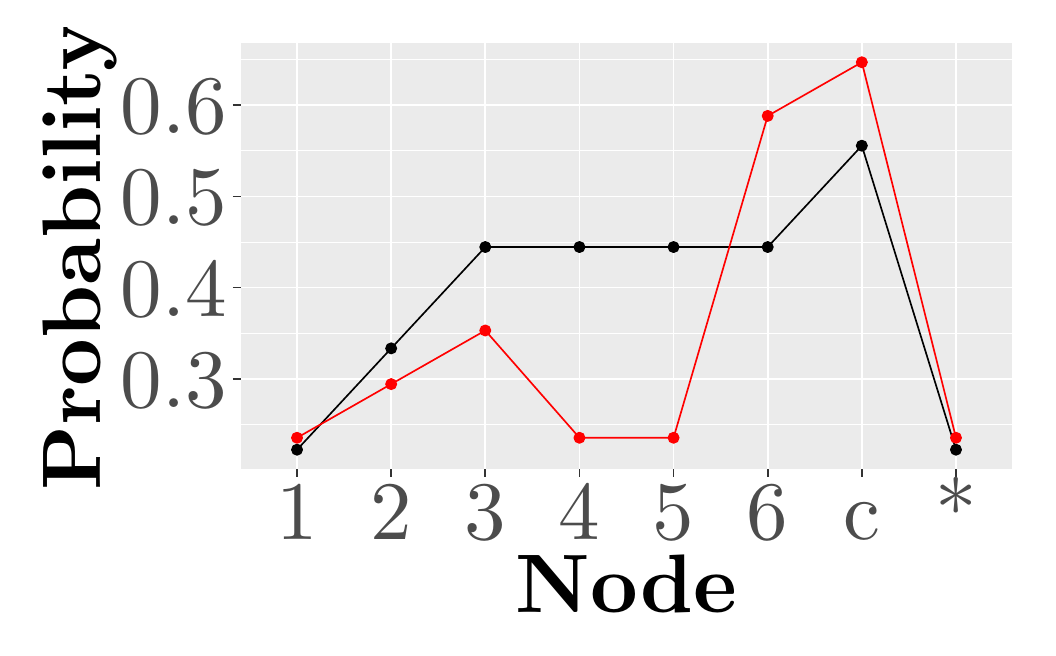
\begin{tikzpicture}[x=1pt,y=1pt]
\definecolor{fillColor}{RGB}{255,255,255}
\path[use as bounding box,fill=fillColor,fill opacity=0.00] (0,0) rectangle (361.35,216.81);
\begin{scope}
\path[clip] (  0.00,  0.00) rectangle (361.35,216.81);
\definecolor{drawColor}{RGB}{255,255,255}
\definecolor{fillColor}{RGB}{255,255,255}

\path[draw=drawColor,line width= 0.6pt,line join=round,line cap=round,fill=fillColor] (  0.00,  0.00) rectangle (361.35,216.81);
\end{scope}
\begin{scope}
\path[clip] ( 76.92, 57.31) rectangle (355.85,211.31);
\definecolor{fillColor}{gray}{0.92}

\path[fill=fillColor] ( 76.92, 57.31) rectangle (355.85,211.31);
\definecolor{drawColor}{RGB}{255,255,255}

\path[draw=drawColor,line width= 0.3pt,line join=round] ( 76.92, 73.47) --
	(355.85, 73.47);

\path[draw=drawColor,line width= 0.3pt,line join=round] ( 76.92,106.42) --
	(355.85,106.42);

\path[draw=drawColor,line width= 0.3pt,line join=round] ( 76.92,139.37) --
	(355.85,139.37);

\path[draw=drawColor,line width= 0.3pt,line join=round] ( 76.92,172.33) --
	(355.85,172.33);

\path[draw=drawColor,line width= 0.3pt,line join=round] ( 76.92,205.28) --
	(355.85,205.28);

\path[draw=drawColor,line width= 0.6pt,line join=round] ( 76.92, 89.94) --
	(355.85, 89.94);

\path[draw=drawColor,line width= 0.6pt,line join=round] ( 76.92,122.90) --
	(355.85,122.90);

\path[draw=drawColor,line width= 0.6pt,line join=round] ( 76.92,155.85) --
	(355.85,155.85);

\path[draw=drawColor,line width= 0.6pt,line join=round] ( 76.92,188.80) --
	(355.85,188.80);

\path[draw=drawColor,line width= 0.6pt,line join=round] ( 97.33, 57.31) --
	( 97.33,211.31);

\path[draw=drawColor,line width= 0.6pt,line join=round] (131.35, 57.31) --
	(131.35,211.31);

\path[draw=drawColor,line width= 0.6pt,line join=round] (165.36, 57.31) --
	(165.36,211.31);

\path[draw=drawColor,line width= 0.6pt,line join=round] (199.38, 57.31) --
	(199.38,211.31);

\path[draw=drawColor,line width= 0.6pt,line join=round] (233.39, 57.31) --
	(233.39,211.31);

\path[draw=drawColor,line width= 0.6pt,line join=round] (267.41, 57.31) --
	(267.41,211.31);

\path[draw=drawColor,line width= 0.6pt,line join=round] (301.42, 57.31) --
	(301.42,211.31);

\path[draw=drawColor,line width= 0.6pt,line join=round] (335.44, 57.31) --
	(335.44,211.31);
\definecolor{drawColor}{RGB}{0,0,0}
\definecolor{fillColor}{RGB}{0,0,0}

\path[draw=drawColor,line width= 0.4pt,line join=round,line cap=round,fill=fillColor] ( 97.33, 64.31) circle (  1.96);

\path[draw=drawColor,line width= 0.4pt,line join=round,line cap=round,fill=fillColor] (131.35,100.93) circle (  1.96);

\path[draw=drawColor,line width= 0.4pt,line join=round,line cap=round,fill=fillColor] (165.36,137.54) circle (  1.96);

\path[draw=drawColor,line width= 0.4pt,line join=round,line cap=round,fill=fillColor] (199.38,137.54) circle (  1.96);

\path[draw=drawColor,line width= 0.4pt,line join=round,line cap=round,fill=fillColor] (233.39,137.54) circle (  1.96);

\path[draw=drawColor,line width= 0.4pt,line join=round,line cap=round,fill=fillColor] (267.41,137.54) circle (  1.96);

\path[draw=drawColor,line width= 0.4pt,line join=round,line cap=round,fill=fillColor] (301.42,174.16) circle (  1.96);

\path[draw=drawColor,line width= 0.4pt,line join=round,line cap=round,fill=fillColor] (335.44, 64.31) circle (  1.96);

\path[draw=drawColor,line width= 0.6pt,line join=round] ( 97.33, 64.31) --
	(131.35,100.93) --
	(165.36,137.54) --
	(199.38,137.54) --
	(233.39,137.54) --
	(267.41,137.54) --
	(301.42,174.16) --
	(335.44, 64.31);
\definecolor{drawColor}{RGB}{255,0,0}
\definecolor{fillColor}{RGB}{255,0,0}

\path[draw=drawColor,line width= 0.4pt,line join=round,line cap=round,fill=fillColor] ( 97.33, 68.62) circle (  1.96);

\path[draw=drawColor,line width= 0.4pt,line join=round,line cap=round,fill=fillColor] (131.35, 88.01) circle (  1.96);

\path[draw=drawColor,line width= 0.4pt,line join=round,line cap=round,fill=fillColor] (165.36,107.39) circle (  1.96);

\path[draw=drawColor,line width= 0.4pt,line join=round,line cap=round,fill=fillColor] (199.38, 68.62) circle (  1.96);

\path[draw=drawColor,line width= 0.4pt,line join=round,line cap=round,fill=fillColor] (233.39, 68.62) circle (  1.96);

\path[draw=drawColor,line width= 0.4pt,line join=round,line cap=round,fill=fillColor] (267.41,184.93) circle (  1.96);

\path[draw=drawColor,line width= 0.4pt,line join=round,line cap=round,fill=fillColor] (301.42,204.31) circle (  1.96);

\path[draw=drawColor,line width= 0.4pt,line join=round,line cap=round,fill=fillColor] (335.44, 68.62) circle (  1.96);

\path[draw=drawColor,line width= 0.6pt,line join=round] ( 97.33, 68.62) --
	(131.35, 88.01) --
	(165.36,107.39) --
	(199.38, 68.62) --
	(233.39, 68.62) --
	(267.41,184.93) --
	(301.42,204.31) --
	(335.44, 68.62);
\end{scope}
\begin{scope}
\path[clip] (  0.00,  0.00) rectangle (361.35,216.81);
\definecolor{drawColor}{gray}{0.30}

\node[text=drawColor,anchor=base east,inner sep=0pt, outer sep=0pt, scale=  3.00] at ( 71.97, 79.61) {0.3};

\node[text=drawColor,anchor=base east,inner sep=0pt, outer sep=0pt, scale=  3.00] at ( 71.97,112.57) {0.4};

\node[text=drawColor,anchor=base east,inner sep=0pt, outer sep=0pt, scale=  3.00] at ( 71.97,145.52) {0.5};

\node[text=drawColor,anchor=base east,inner sep=0pt, outer sep=0pt, scale=  3.00] at ( 71.97,178.47) {0.6};
\end{scope}
\begin{scope}
\path[clip] (  0.00,  0.00) rectangle (361.35,216.81);
\definecolor{drawColor}{gray}{0.20}

\path[draw=drawColor,line width= 0.6pt,line join=round] ( 74.17, 89.94) --
	( 76.92, 89.94);

\path[draw=drawColor,line width= 0.6pt,line join=round] ( 74.17,122.90) --
	( 76.92,122.90);

\path[draw=drawColor,line width= 0.6pt,line join=round] ( 74.17,155.85) --
	( 76.92,155.85);

\path[draw=drawColor,line width= 0.6pt,line join=round] ( 74.17,188.80) --
	( 76.92,188.80);
\end{scope}
\begin{scope}
\path[clip] (  0.00,  0.00) rectangle (361.35,216.81);
\definecolor{drawColor}{gray}{0.20}

\path[draw=drawColor,line width= 0.6pt,line join=round] ( 97.33, 54.56) --
	( 97.33, 57.31);

\path[draw=drawColor,line width= 0.6pt,line join=round] (131.35, 54.56) --
	(131.35, 57.31);

\path[draw=drawColor,line width= 0.6pt,line join=round] (165.36, 54.56) --
	(165.36, 57.31);

\path[draw=drawColor,line width= 0.6pt,line join=round] (199.38, 54.56) --
	(199.38, 57.31);

\path[draw=drawColor,line width= 0.6pt,line join=round] (233.39, 54.56) --
	(233.39, 57.31);

\path[draw=drawColor,line width= 0.6pt,line join=round] (267.41, 54.56) --
	(267.41, 57.31);

\path[draw=drawColor,line width= 0.6pt,line join=round] (301.42, 54.56) --
	(301.42, 57.31);

\path[draw=drawColor,line width= 0.6pt,line join=round] (335.44, 54.56) --
	(335.44, 57.31);
\end{scope}
\begin{scope}
\path[clip] (  0.00,  0.00) rectangle (361.35,216.81);
\definecolor{drawColor}{gray}{0.30}

\node[text=drawColor,anchor=base,inner sep=0pt, outer sep=0pt, scale=  3.00] at ( 97.33, 31.70) {1};

\node[text=drawColor,anchor=base,inner sep=0pt, outer sep=0pt, scale=  3.00] at (131.35, 31.70) {2};

\node[text=drawColor,anchor=base,inner sep=0pt, outer sep=0pt, scale=  3.00] at (165.36, 31.70) {3};

\node[text=drawColor,anchor=base,inner sep=0pt, outer sep=0pt, scale=  3.00] at (199.38, 31.70) {4};

\node[text=drawColor,anchor=base,inner sep=0pt, outer sep=0pt, scale=  3.00] at (233.39, 31.70) {5};

\node[text=drawColor,anchor=base,inner sep=0pt, outer sep=0pt, scale=  3.00] at (267.41, 31.70) {6};

\node[text=drawColor,anchor=base,inner sep=0pt, outer sep=0pt, scale=  3.00] at (301.42, 31.70) {c};

\node[text=drawColor,anchor=base,inner sep=0pt, outer sep=0pt, scale=  3.00] at (335.44, 31.70) {*};
\end{scope}
\begin{scope}
\path[clip] (  0.00,  0.00) rectangle (361.35,216.81);
\definecolor{drawColor}{RGB}{0,0,0}

\node[text=drawColor,anchor=base,inner sep=0pt, outer sep=0pt, scale=  3.00] at (216.39,  5.50) {\bfseries Node};
\end{scope}
\begin{scope}
\path[clip] (  0.00,  0.00) rectangle (361.35,216.81);
\definecolor{drawColor}{RGB}{0,0,0}

\node[text=drawColor,rotate= 90.00,anchor=base,inner sep=0pt, outer sep=0pt, scale=  3.00] at ( 26.20,134.31) {\bfseries Probability};
\end{scope}
\end{tikzpicture}
